\begin{figure}
\centering
%\mbox{
  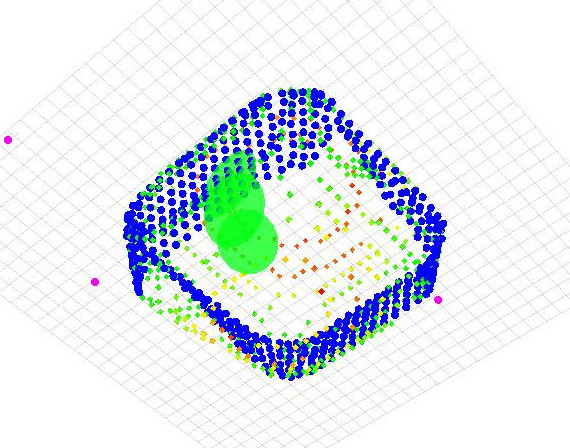
\includegraphics[width=0.9\linewidth]{next_best_touch.jpg}
  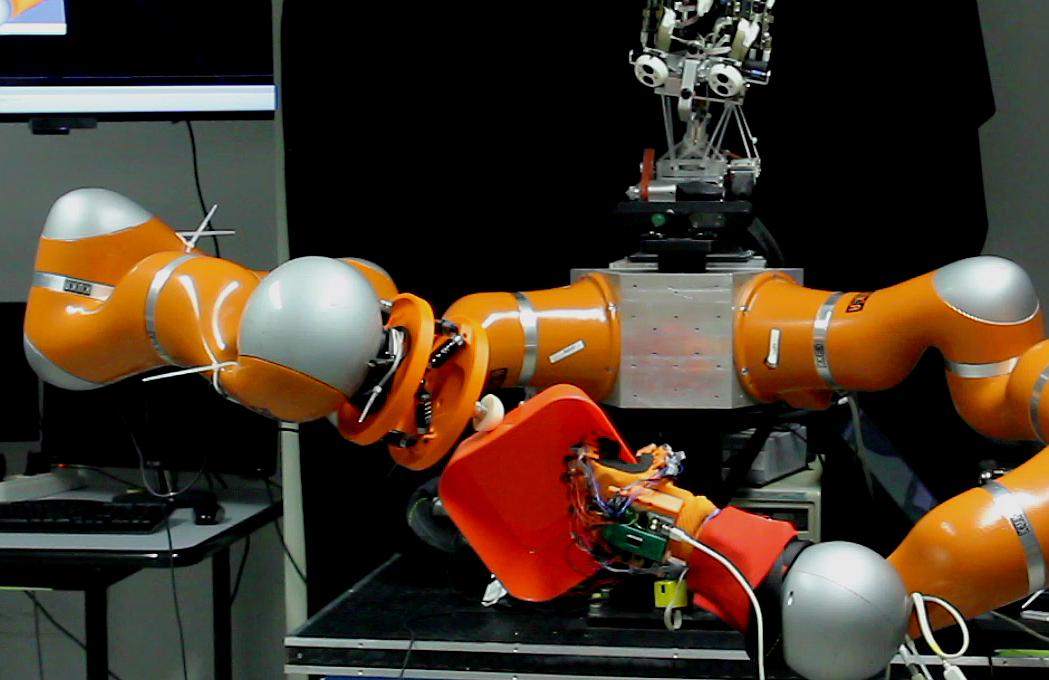
\includegraphics[width=0.7\linewidth]{intro_vito.png}
%}
\caption{The GPAtlasRRT strategy suggests a touch(es) (lighter green colored disks) on the predicted surface. The predicted surface is shown in points colored from green to red according to higher or lower variance of the prediction, respectively, and the blue points are the initial partial view (left). Our Vito robot executes it as a tactile exploration (right). }
\label{fig:setup_solution}
\end{figure}

% why the problem we are dealing with is important
One of the main reasons that makes autonomous grasping tasks, an ubiquitous and fundamental task in robotics, very challenging is that object properties required for grasp planning like shape and friction are not known %\emph{a priori}.
in advance.
This requires robots to perceive objects around them based on sensory information. However, sensory systems are prone to errors. As an example, when considering vision, some sources of noise are imperfect scene segmentation, occlusions, and poor lighting conditions.

Although for robotic grasp planning the use of vision has been studied more in depth by~\cite{Kragic2002TechRep}, the superior capabilities of humans in interacting with the environment come from rich sensory information where both visual and haptic modalities contribute to the combined percept. Working toward this ability in robots, the goal of our work is to complement visual information with tactile sensing in order to acquire 3D object models.

Even if tactile perception needs have been authoritatively spelled out by \cite{Bajcsy1988Active} in the 1980's and early perception algorithms date back to the same years \citep{Grimson1984JRR,Faugeras1983IJCAI,Shekhar1986ICRA,Bajcsy1989Machine}, touch-based perception has lagged behind vision for two main reasons. The first is technological: standardized touch sensors are not easily available and have to be hand crafted for the specific robot and task. The second is intrinsic to the perception modality which requires the mechanical interaction of the sensor with the object being perceived with its inevitable perturbation and, to minimize this effect, calls for a complex control of the ongoing movement of the sensor: a requirement which is completely absent, e.g., in vision.

The scenario we pursue is motivated by tactile exploration when other sensor modalities, like vision, already provided initial and incomplete information on object shape. More in details, we provide a systematic methodology to plan the next-best tactile exploration action. This is intrinsically a contact hypothesis that needs to be accepted or discarded after execution. Despite being the hypothesis verified or falsified, it helps to improve the object shape prediction up to a pre-specified variability.

The object shape representation we employ is a probabilistic one and it is based on Gaussian Process (GP) \citep{Rasmussen2006Gaussian}, a machine learning formalism for nonlinear function regression that naturally provides a quantification of multi-modal uncertainty about object point estimates, i.e. the variance of the estimate. Being the $0$-levelset of an \emph{unknown} function an implicitly defined surface that represents the estimated outer shape of an object, it comes handy to interpret it as a manifold and build on recent results on sample-based exploration of general manifolds~\citep{Jaillet2013Path}, and implement similar algorithms to define hypotheses on where to sample next --- next-best touch --- to reduce uncertainty. More in details, without the need to embed the manifold in its ambient space, we build a collection of charts (atlas) that locally parameterizes it, and select among the points on the current atlas the one(s) fulfilling the search criteria: this represents the location where the next touch will be directed. Then, the growth of the atlas itself does not follow a predefined sequence of steps, but an RRT-like strategy is employed to devise random directions to expand the atlas.
We propose a search criteria that looks for points on the estimated surface with the variance of being there larger than a pre-specified threshold. From another point of view, we look in all for an estimated surface, such that, any arbitrary point on it has a variance smaller than the pre-specified threshold. The expansion process is then repeated iteratively after the execution of the suggested touch.
It certainly trades completeness in the novel shape exploration for efficiency: the RRT drives the growth of the atlas toward  regions of the object surface that are more uncertain, delaying the refinement of areas that have been already explored.

The ending condition is met when no candidate for the next best touch is found by the GPAtlasRRT algorithm, which means the that object shape prediction meets the requirement on variability.
Naturally, the smaller the threshold (i.e. a more accurate model is required), the higher the number of touches. This is the only input to the devised strategy, given either by a higher level module or the user.

The structure of the paper is described in the following: in Sec.~\ref{sec:related} we first review previous work related to tactile exploration and object shape representations. In Sec.~\ref{sec:scope} we clearly state the problem we aim to solve and in Sec.~\ref{sec:solution} we present the envisioned approach for its solution. The experimental results and their discussion are presented in Sec.~\ref{sec:experiments}. Finally, conclusions and points deserving further attention are given in Sec.~\ref{sec:conclusions}.

% why tactile exploration is not so developed
% and what makes the problem harder that active vision

% why we propose touch (Bajcsy) and why ITS

% what is exactly our contribution

% RELATED WORK

% only localization

% also shape reconstruction
% they also use GP

% what are we doing more at least in surface exploration?
% we are exploiting the implicit manifold nature of GP representation
% and adapt efficient sample-based method for exploring the manifold in
% an intrinsic  way.



%General guidelines : \citet{Bajcsy1989Machine}
%
%Active visual perception: \citet{Bajcsy1988Active}
%
%Vision-based exploration is the most studied, perhaps due to its non-invasive nature, which avoids the contact between rigid bodies which is the cause of most headaches in physics modelling, simulation and control.
%
%As very well said by \citet{Petrovskaya2011Global}, even when initial works date back to the 80's, tactile perception has not been addressed as deeply as the non-invasive counterpart, visual perception. Besides the need of being actively controlled, tactile sensors typically required ad-hoc mechanical devices.
%
%``Touch-based perception has not been studied in as much depth
%as vision because standardized touch sensors are not as easily
%available. In many situations, tactile sensors have to be hand
%crafted specifically for the robot and the task. This complicates
%comparisons between methods and slows progress in tactile
%perception. However, recently there has been a surge of interest
%in the field due to the necessity of touch-based perception in
%service applications''
%
%Whereas \citet{Petrovskaya2011Global} is more interested in the object pose estimation problem, here we are more interested in the object shape modelling, sort of in the mapping of rather than localization in a SLAM problem.
%
%On active touch sensing \citet{Prescott2011Active}
%
%Differentiate from active touch for localization, here another example: \citet{Hebert2013Next}.
%
%Justify the use of a intrinsic tactile sensor over a tactile array.
%
%ITS are more precise and less noisy. It provides the contact normal directly in sensor frame.
%
%Tactile arrays provide multiple-point measurements. They do not provide directly the normal in sensor frame, forward kinematics is required over noisy joint measurements, or in fixed configurations that limit exploration mobility. Up to a point that a typically a complex framework is needed to exploit its grasping and touching properties % cite http://www.roboticsproceedings.org/rss09/p45.pdf?
%
%With ITS, the computation will be trivial. The disadvantage is that it is a single-point measurement. Poking strategies, like in~\citet{Petrovskaya2011Global}, or trajectories strategies like in~\citet{Rosales2014Active}.
%
%% They claim that touch sensing is low bandwith, local, sequential process with better signal-to-noise ratio than vision.
%
%% Vision is global, has high bandwidth, and is noisy. Touch is a low bandwidth, local, sequential process with better noise properties than vision.
%
%%% Finish the introduction with some motivation
%On how to do classification...
%
%Shape representation and descriptor review \citet{Zhang2004Review}
%
%In this work, we provide a systematic methodology to plan the next-best tactile exploratory action. The tactile exploratory action is intrinsically a contact hypothesis that need to be accepted or discarded after execution. Should the result be any of the two, it helps to improve the object shape prediction up to a pre-specified variability. In contrast to \citet{Bjorkman2013Enhancing}, we propose the same shape representation as descriptor for classification purposes using shape matching techniques~\citep{Belongie2002Shape}. The scope and problem statement is detailed in Sect.~\ref{sec:scope}. The proposed solution is broaden in Sect.~\ref{sec:solution}. The experimental results and discusion is presented in Sect.~\ref{sec:experiments}. Finally, the conclusions and points deserving further attention as given in Sect.~\ref{sec:conclusions}.
%%Reading the paper along watching the attached media is suggested for a better cath-up of the ideas. 